\begin{frame}{Attuazione}
\begin{columns}

\column{0.5\textwidth}
\begin{itemize}
    \item<1-> estrinseca
    \begin{itemize}
        \item <3-> nelle strutture multi-backbone
        \item <4-> nelle strutture a tubi concentrici
    \end{itemize}
    \item<2-> intrinseca
    \begin{itemize}
        \item<5-> attraverso camera idraulica
        \item<6-> attraverso shape memory effect
        \item<7-> attraverso micro-motori
        \item<8-> attraverso campi magnetici generati da MRI
    \end{itemize}
\end{itemize}

\column{0.5\textwidth}
\only<1-2>{
\includegraphics[height=0.7\textheight]{slide_studio/img_attuazione/attuazione_none.png}}
\only<3>{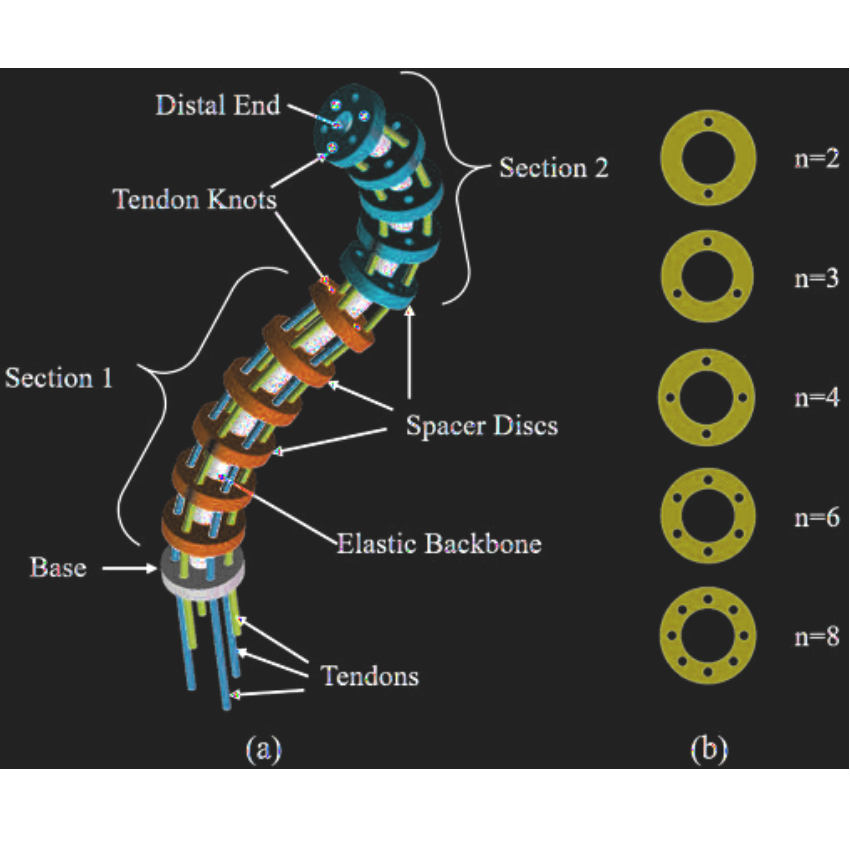
\includegraphics[height=0.7\textheight]{slide_studio/img_attuazione/attuazione_ext_multibackbone.png}}
\only<4>{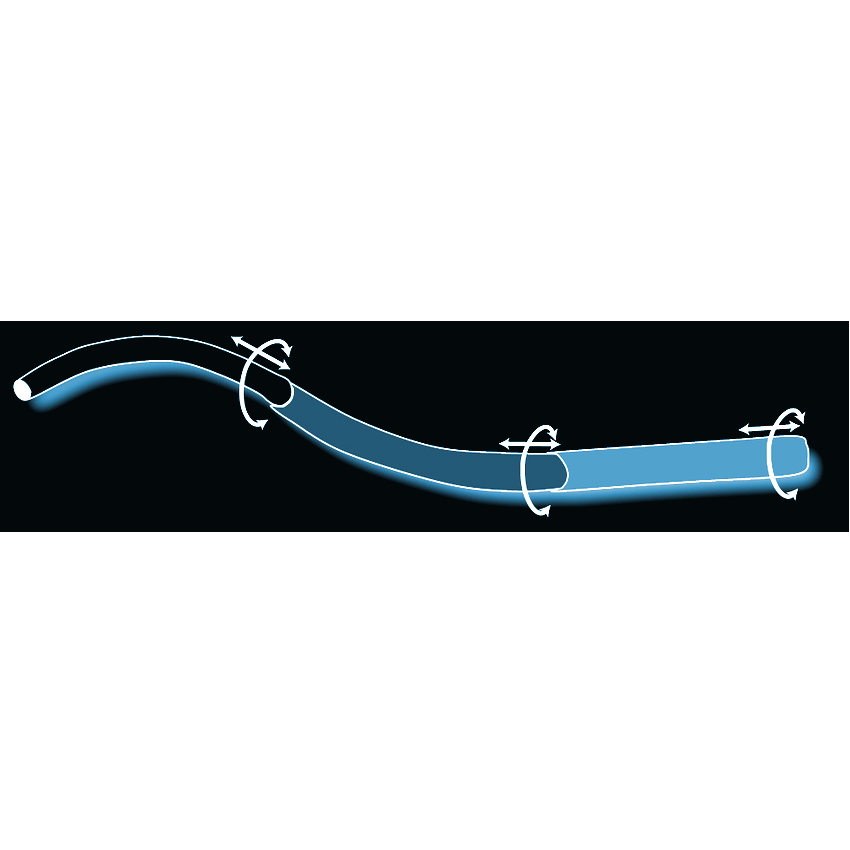
\includegraphics[height=0.7\textheight]{slide_studio/img_attuazione/attuazione_ext_concentrico.png}}
\only<5>{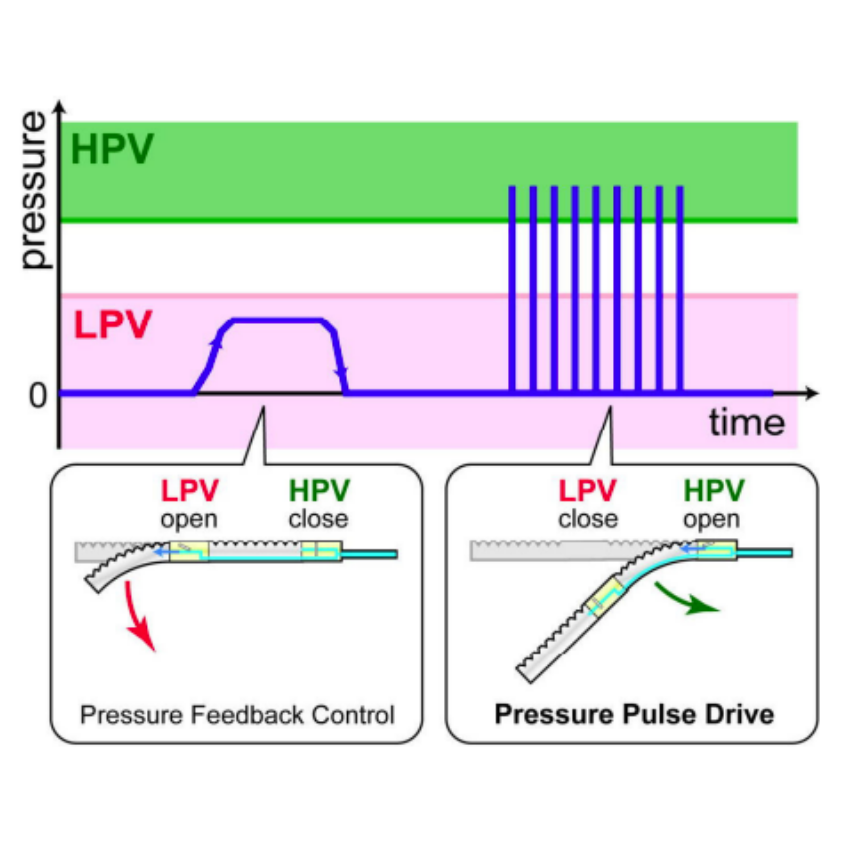
\includegraphics[height=0.7\textheight]{slide_studio/img_attuazione/attuazione_int_valvole.png}}
\only<6>{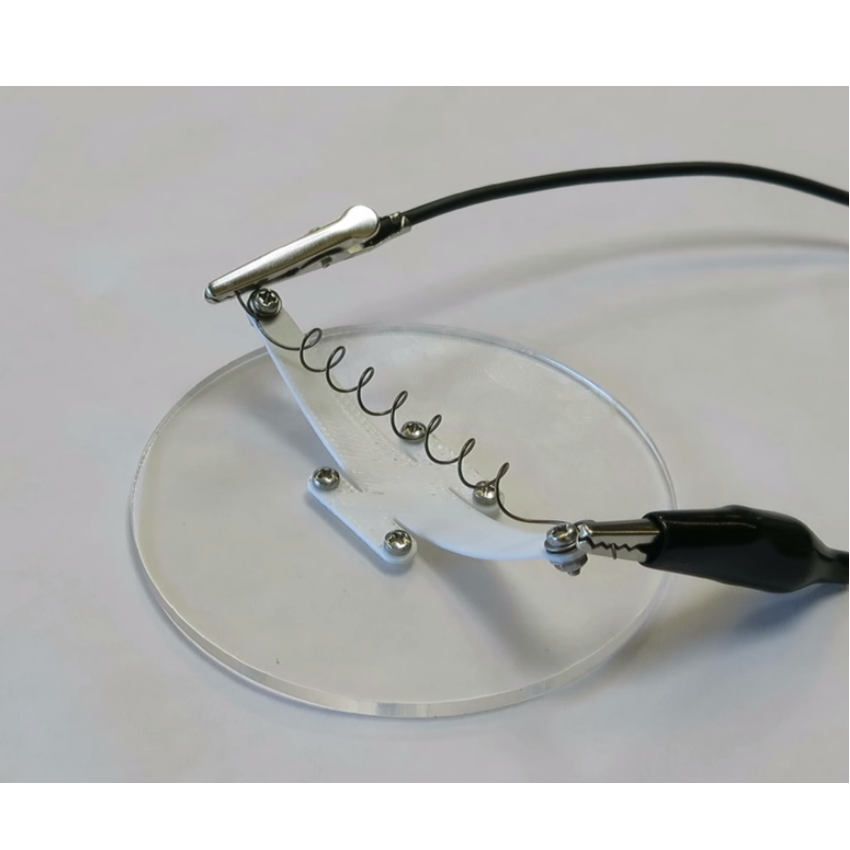
\includegraphics[height=0.7\textheight]{slide_studio/img_attuazione/attuazione_int_shapememory.png}}
\only<7>{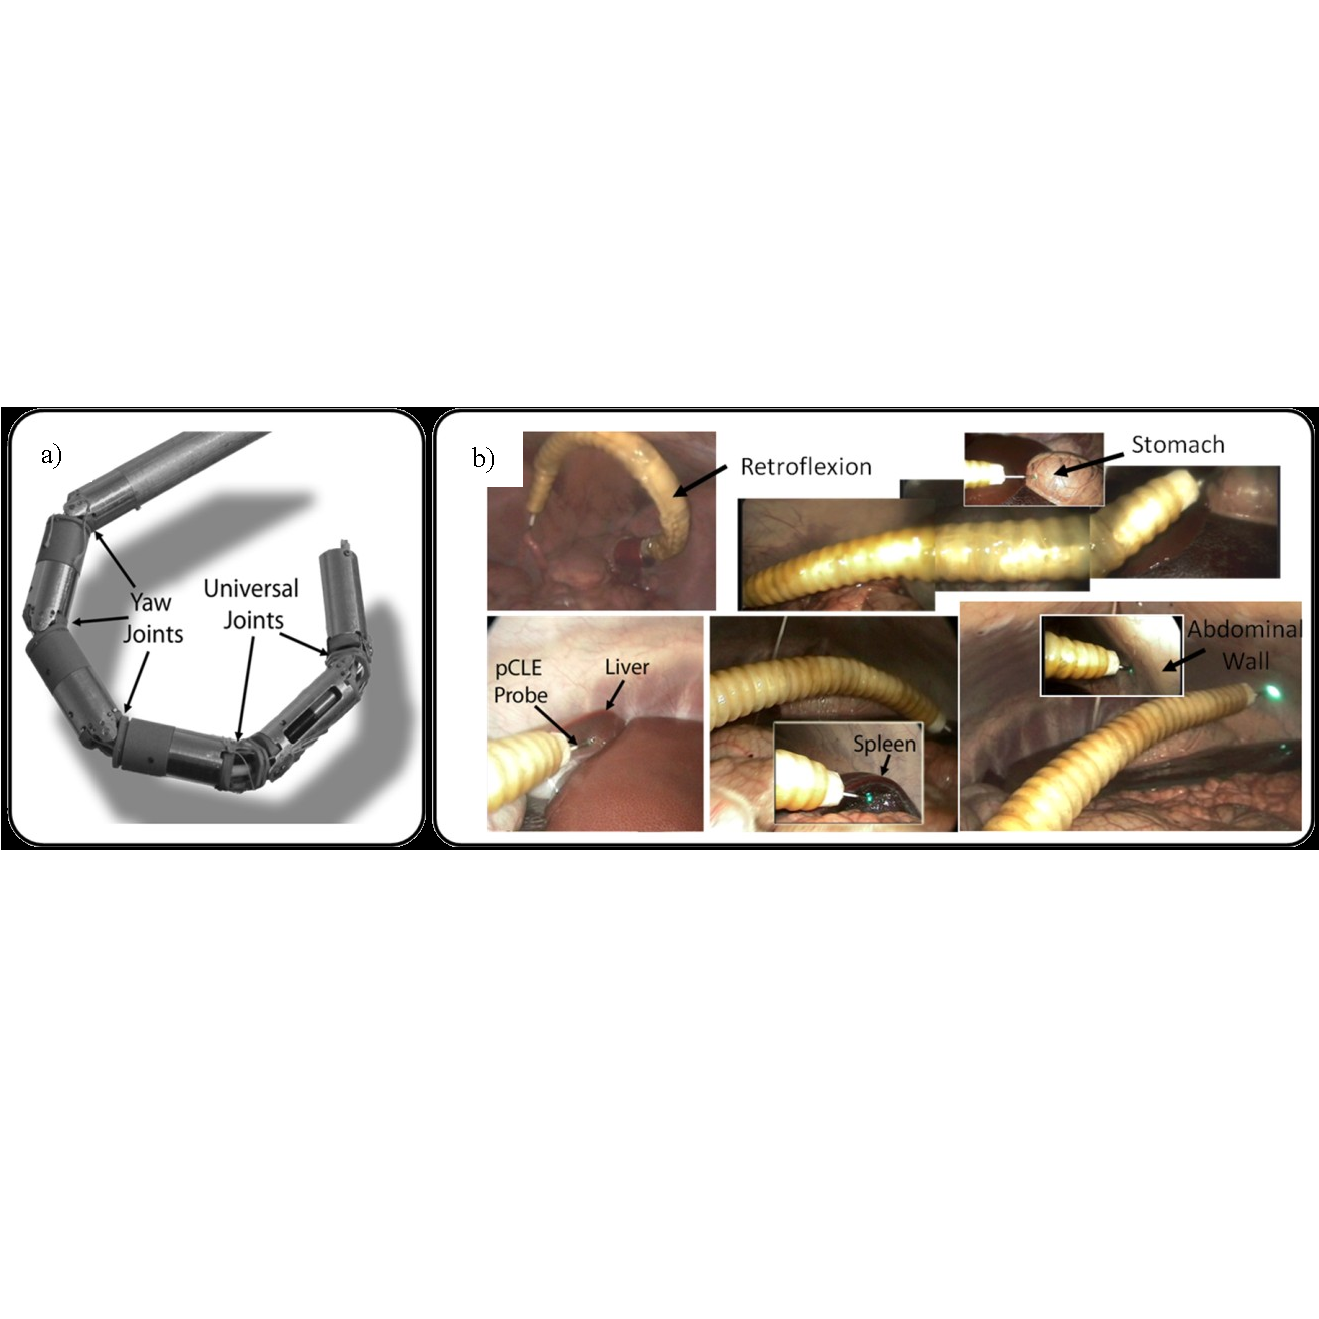
\includegraphics[height=0.7\textheight]{slide_studio/img_attuazione/attuazione_int_motori.png}}
\only<8>{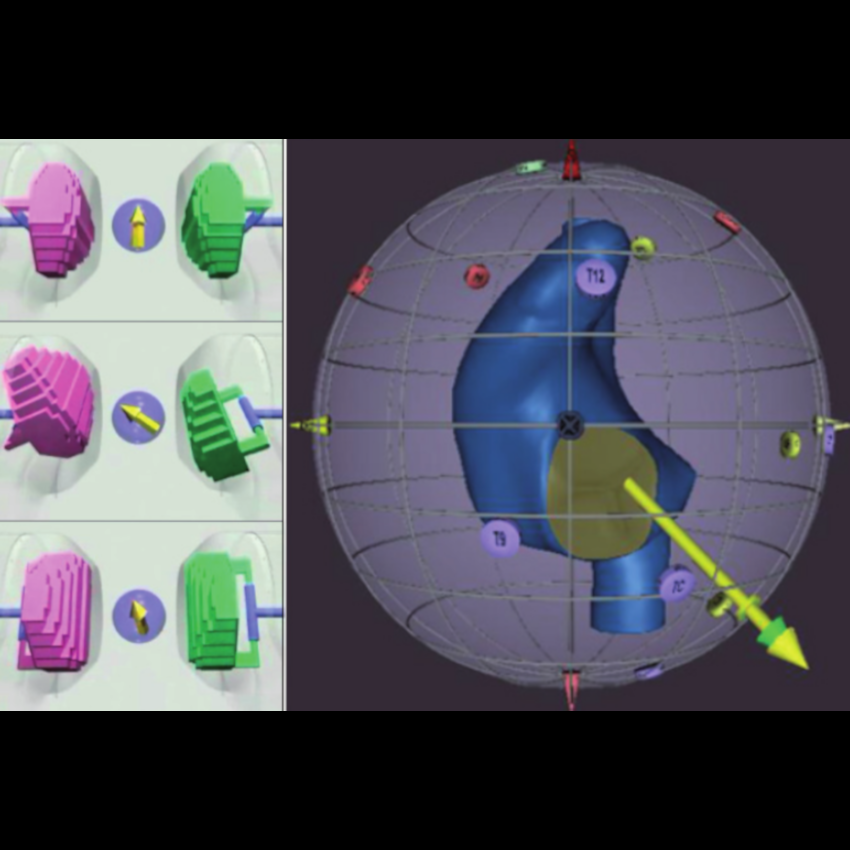
\includegraphics[height=0.7\textheight]{slide_studio/img_attuazione/attuazione_int_mri.png}}

\end{columns}

\only<3>{\Reference{Kinematic comparison of surgical tendon-driven manipulators and concentric tube manipulators}{Li, Wu, Ren, You}{2017}}
\only<4>{\Reference{Workspace characterization for concentric tube continuum robots}{Burgner-Kahrs et al.}{2014}}
\only<5>{\Reference{Precise Bending Angle Control of Hydraulic Active Catheter by Pressure Pulse Drive}{Ikuta et al.}{2010}}
\only<6>{\Reference{Clip ``SMA actuator design"}{\url{https://www.youtube.com/watch?v=PxBPpPRkv6A}}{2015}}
\only<7>{\Reference{A modular, mechatronic joint design for a flexible access platform for MIS}{Noonan et al.}{2011}}
\only<8>{\Reference{Stereotaxis Niobe magnetic navigation system for endocardial catheter ablation and gastrointestinal capsule endoscopy}{Carpi, Pappone}{2009}}

\note{
Attuazione $\to$ punto in cui la potenza viene convertita in energia meccanica. 

Estrinseca $\to$ fuori dalla struttura (diametro robot minore). 

Intrinseca $\to$ dentro la struttura (minore frizione, minore footprint in sala operatoria).

Estrinseca multibackbone $\to$ tendini, cavi da tirare per dare la curvatura desiderata. 

Estrinseca tubi concentrici $\to$ ruoto e traslo base dei tubi per controllare forma del robot. 
Intrinseco idrulico $\to$ valvole che si aprono ad uno specifico range di pressione (driving range). Il liquido confluisce in una o l'altra direzione, muovendo il manipolatore. 

Intrinseco shape memory $\to$ proprietà delle leghe metalliche. Il materiale si deforma sottoposto ad un carico, torna alla forma originale se riscaldato. 

Intrinseco micro-motori $\to$ devono essere piccoli. 

Intrinseco MRI $\to$ usato nei cateteri con punta magnetica. Viene mosso da campo magnetico generato da una macchina simile allo scanner MRI.
}
\end{frame}
